% Sustentación del Taller 3 (tema Beamer institucional UD). Compilar:  make slides
% Las cifras (\cifra...) salen de ../informe/numeros.tex, generado por desarrollo/exportar_informe.py.
\documentclass[aspectratio=169,10pt]{beamer}
\usepackage[spanish,es-noshorthands]{babel}
\usetheme{UD}
% Generado por desarrollo/exportar_informe.py: NO editar a mano.
\newcommand{\cifraaugLoteVal}{0,00}
\newcommand{\cifraaugLoteValGana}{1}
\newcommand{\cifraaugLoteTe}{$-$0,33}
\newcommand{\cifraaugLoteTeGana}{1}
\newcommand{\cifraaugMuestraVal}{0,12}
\newcommand{\cifraaugMuestraValGana}{3}
\newcommand{\cifraaugMuestraTe}{$-$0,25}
\newcommand{\cifraaugMuestraTeGana}{1}
\newcommand{\cifraaugN}{5}
\newcommand{\cifralargoValDif}{$-$0,15}
\newcommand{\cifralargoTeDif}{$-$0,19}
\newcommand{\cifralargoBrechaSin}{1,09}
\newcommand{\cifralargoBrechaCon}{0,40}
\newcommand{\cifraablBnTe}{0,54}
\newcommand{\cifraablBnVal}{0,32}
\newcommand{\cifraablBnBrecha}{0,83}
\newcommand{\cifraablDropTe}{$-$0,52}
\newcommand{\cifraablDropVal}{$-$0,47}
\newcommand{\cifraablDropBrecha}{1,45}
\newcommand{\cifraablAmbosTe}{0,46}
\newcommand{\cifraablAmbosVal}{0,11}
\newcommand{\cifraablAmbosBrecha}{1,46}
\newcommand{\cifraablTresTe}{2,11}
\newcommand{\cifraablTresVal}{1,07}
\newcommand{\cifraablTresBrecha}{0,89}
\newcommand{\cifraablBrechaCompleta}{0,90}
\newcommand{\ciframlpTe}{88,44}
\newcommand{\cifracnnDocTe}{91,20}
\newcommand{\cifracnnPropTe}{92,10}
\newcommand{\cifracnnPropVsMlp}{3,66}
\newcommand{\cifracnnPropVsDoc}{0,90}
\newcommand{\cifradsMNISTTe}{98,80}
\newcommand{\cifradsMNISTVal}{98,72}
\newcommand{\cifradsMNISTGap}{$-$0,1}
\newcommand{\cifradsMNISTPeor}{97,2}
\newcommand{\cifradsMNISTBajo}{0,0}
\newcommand{\cifradsFashionMNISTTe}{90,27}
\newcommand{\cifradsFashionMNISTVal}{90,34}
\newcommand{\cifradsFashionMNISTGap}{0,1}
\newcommand{\cifradsFashionMNISTPeor}{72,2}
\newcommand{\cifradsFashionMNISTBajo}{4,3}
\newcommand{\cifradsKMNISTTe}{92,10}
\newcommand{\cifradsKMNISTVal}{97,15}
\newcommand{\cifradsKMNISTGap}{5,1}
\newcommand{\cifradsKMNISTPeor}{86,3}
\newcommand{\cifradsKMNISTBajo}{2,0}
\newcommand{\cifralrUno}{82,46}
\newcommand{\cifralrSinBnUno}{9,76}
\newcommand{\cifralrDos}{96,70}
\newcommand{\cifralrSinBnDos}{92,62}
\newcommand{\cifralrTres}{96,30}
\newcommand{\cifralrSinBnTres}{96,52}
\newcommand{\cifralrCuatro}{92,38}
\newcommand{\cifralrCinco}{76,30}
\newcommand{\cifraaccTest}{91,85}
\newcommand{\cifraaccVal}{97,40}
\newcommand{\cifraaccTr}{96,31}
\newcommand{\cifraerrTest}{815}
\newcommand{\cifralossIni}{0,374}
\newcommand{\cifralossFin}{0,117}
\newcommand{\cifraepocas}{5}
\newcommand{\cifraparA}{su}
\newcommand{\cifraparB}{tsu}
\newcommand{\cifraparN}{60}
\newcommand{\cifraparInv}{21}
\newcommand{\cifraclaseMejor}{tsu}
\newcommand{\cifraclaseMejorAcc}{96,5}
\newcommand{\cifraclasePeor}{su}
\newcommand{\cifraclasePeorAcc}{82,2}
\newcommand{\cifrabrechaValTest}{5,5}


\newcommand{\pts}{\,pts}
\newcommand{\cifraGrande}[3]{\begin{minipage}[t]{0.3\linewidth}\centering
  {\cambriafont\fontsize{14pt}{16pt}\selectfont\bfseries\color{#3}#1\par}{\fontsize{7pt}{8.5pt}\selectfont\color{UDSilver}#2\par}\end{minipage}}

\begin{document}

\UDportada{Redes convolucionales sobre KMNIST}
          {Taller 3: aprendizaje profundo}
          {Juan Felipe Rodríguez Galindo\\{\fontsize{6.4pt}{7.4pt}\selectfont\mdseries\color{UDSilver}20261595004}}
          {Maestría en Ciencias de la Información y las Comunicaciones}
          {Inteligencia Computacional Aplicada}

%% ------------------------------------------------------------------ 2
\begin{frame}{Qué se pidió y qué se hizo}{Mismo flujo del cuaderno del docente, con otro conjunto de datos}
  \begin{columns}[T,onlytextwidth]
    \begin{column}{0.32\textwidth}
      \UDCard{white}{UDBorder}{\cardtitle{UDBlue}{Núcleo (TODO 1 a 5)}{\fontsize{7.5pt}{9.2pt}\selectfont
        Conteo por clase, \texttt{CNNPropia} ($<$ 200\,000 parám.), bucle de entrenamiento, evaluación y par más confundido, aumento de datos.
        Todas las verificaciones en \texttt{[OK]}.\par}}
    \end{column}
    \begin{column}{0.32\textwidth}
      \UDCard{UDLightGray}{UDGold}{\cardtitle{UDGold}{Extras}{\fontsize{7.5pt}{9.2pt}\selectfont
        5 semillas con comparación pareada, ablación y profundidad, líneas base (MLP y CNN del docente), KMNIST vs MNIST vs FashionMNIST, barrido de $\eta$, filtros y mapas.\par}}
    \end{column}
    \begin{column}{0.32\textwidth}
      \UDCard{UDLightGray}{UDRed!60}{\cardtitle{UDRed}{Hallazgo central}{\fontsize{7.5pt}{9.2pt}\selectfont
        En KMNIST la prueba es más difícil que la validación (\cifrabrechaValTest\pts). El aumento de datos \textbf{no} mejoró la exactitud; un tercer bloque sí (\cifraablTresTe\pts).\par}}
    \end{column}
  \end{columns}
  \vspace{0.35cm}
  \begin{center}
  \begin{tikzpicture}[node distance=0.28cm]
    \node[paso] (a) {\textbf{KMNIST}\\60\,000 + 10\,000};
    \node[paso, right=of a] (b) {\textbf{CNNPropia}\\20\,586 parám.};
    \node[paso, right=of b] (c) {\textbf{Adam}\\$\eta=10^{-3}$, \cifraepocas{} ép.};
    \node[paso, right=of c, fill=UDRed!8, draw=UDRed] (d) {\textbf{\cifraaccTest\,\%}\\en prueba};
    \draw[flecha] (a) -- (b); \draw[flecha] (b) -- (c); \draw[flecha] (c) -- (d);
  \end{tikzpicture}
  \end{center}
  \note{Guion: el taller pedía repetir el flujo del docente con KMNIST. Además de los TODO se hicieron extras para responder preguntas abiertas.}
\end{frame}

%% ------------------------------------------------------------------ 3
\begin{frame}{Datos y protocolo}{KMNIST: hiragana cursivo (\textit{kuzushiji}), 10 clases, $28\times28$}
  \begin{columns}[T,onlytextwidth]
    \begin{column}{0.52\textwidth}
      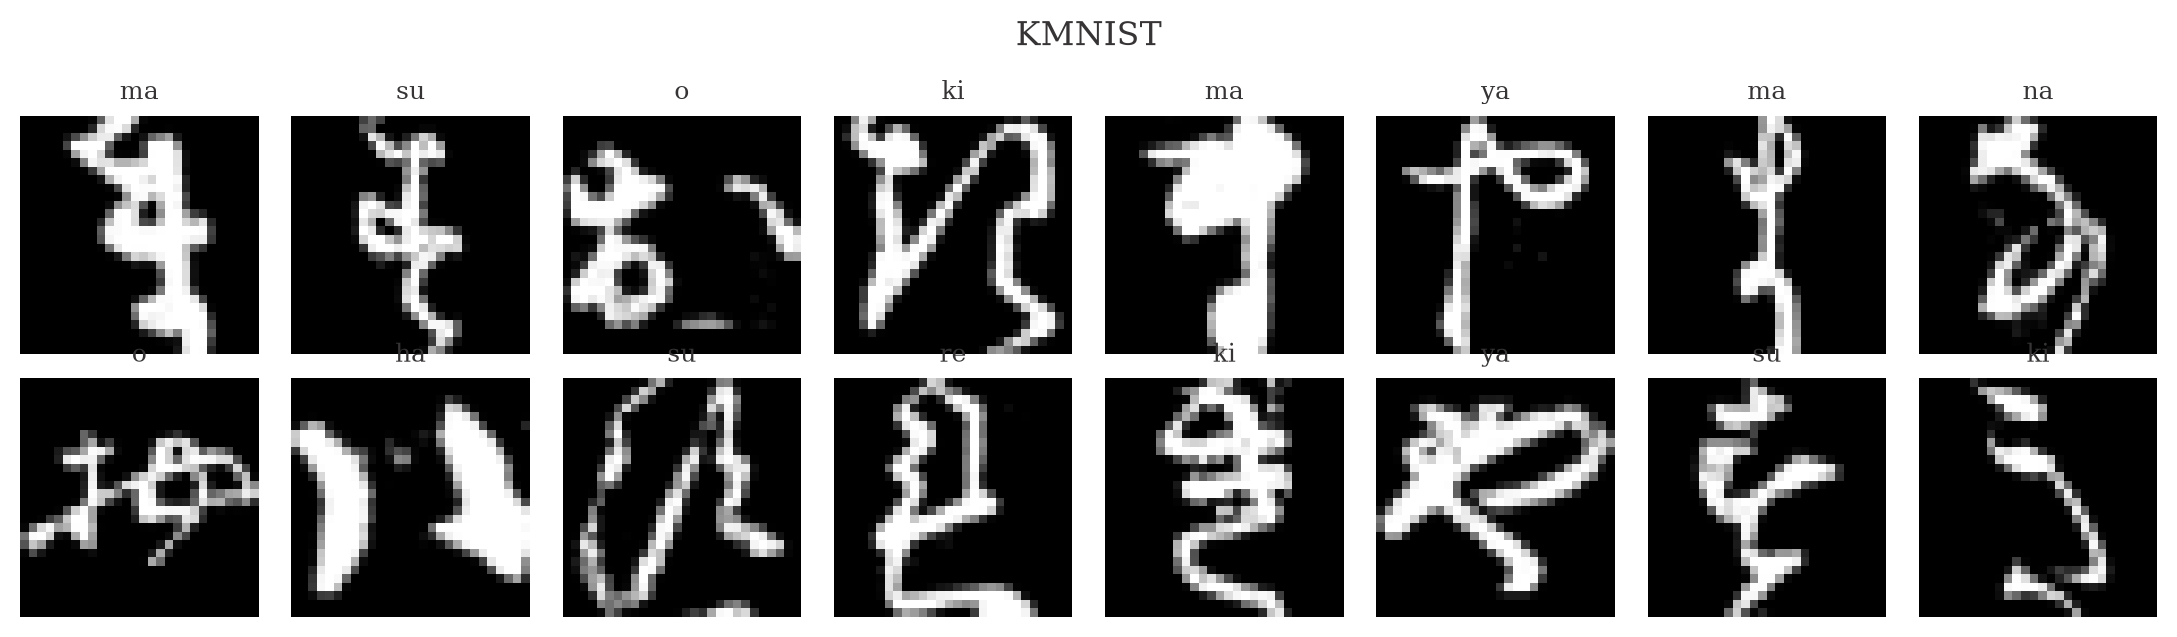
\includegraphics[width=\linewidth]{figuras/f01_muestras.png}\par\vspace{0.1cm}
      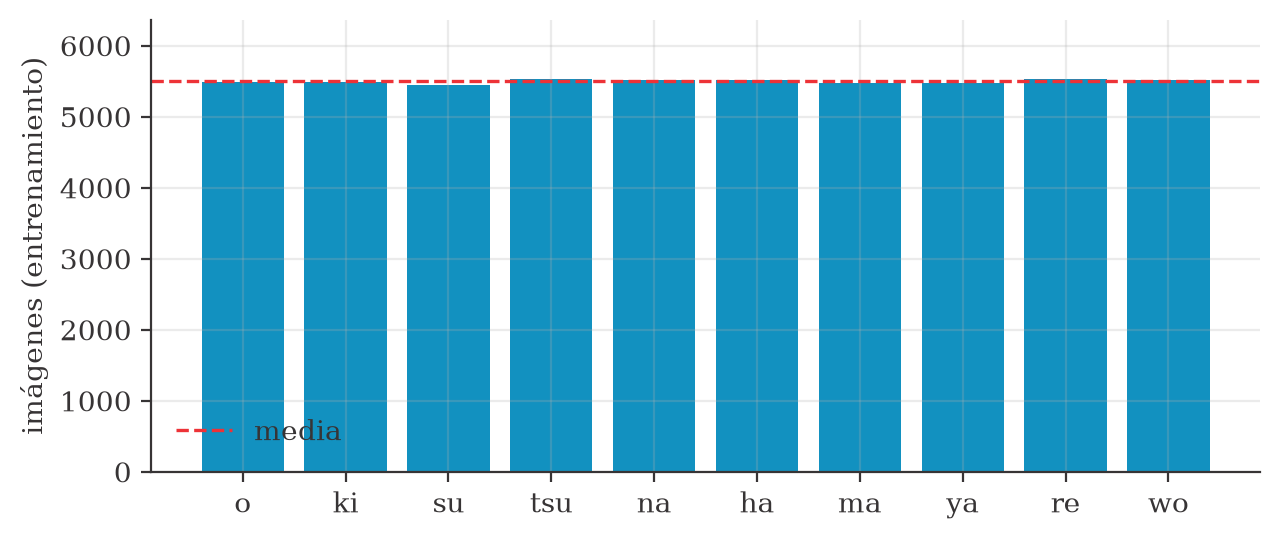
\includegraphics[width=0.9\linewidth]{figuras/f02_conteo_clases.png}
    \end{column}
    \begin{column}{0.45\textwidth}
      \UDCard{white}{UDBorder}{\cardtitle{UDBlue}{Partición}{\fontsize{7.5pt}{9.2pt}\selectfont
        55\,000 entrenamiento / 5\,000 validación / 10\,000 prueba. Normalización con $\mu$ y $\sigma$ \textbf{solo del entrenamiento}. Clases balanceadas (razón máx/mín 1,015).\par}}
      \vspace{0.12cm}
      \UDCard{UDLightGray}{UDGold}{\cardtitle{UDGold}{Comparaciones pareadas}{\fontsize{7.5pt}{9.2pt}\selectfont
        El \texttt{DataLoader} del cuaderno base comparte un generador entre corridas: ``la misma semilla'' no repetía el orden de lotes. Aquí hay un cargador por corrida y 3 a 5 semillas.\par}}
    \end{column}
  \end{columns}
\end{frame}

%% ------------------------------------------------------------------ 4
\begin{frame}{CNNPropia: 20\,586 parámetros}{Dos bloques Conv--BN--ReLU--Pool, Dropout y capa lineal}
  \begin{center}
  \begin{tikzpicture}[node distance=0.22cm]
    \node[paso, text width=1.35cm] (a) {\textbf{Imagen}\\$1{\times}28{\times}28$};
    \node[paso, text width=1.55cm, right=of a, fill=UDBlue!8, draw=UDBlue] (b) {\textbf{Conv 3$\times$3} (16)\\BN + ReLU\\Pool 2$\times$2};
    \node[paso, text width=1.55cm, right=of b, fill=UDBlue!8, draw=UDBlue] (c) {\textbf{Conv 3$\times$3} (32)\\BN + ReLU\\Pool 2$\times$2};
    \node[paso, text width=1.35cm, right=of c] (d) {\textbf{Aplanar}\\Dropout 0,3\\1\,568};
    \node[paso, text width=1.35cm, right=of d, fill=UDRed!8, draw=UDRed] (e) {\textbf{Lineal}\\10 logits};
    \foreach \x/\y in {a/b,b/c,c/d,d/e} \draw[flecha] (\x) -- (\y);
    \node[font=\fontsize{6.5pt}{8pt}\selectfont, text=UDSilver, below=0.05cm of b] {160 + 32 par.};
    \node[font=\fontsize{6.5pt}{8pt}\selectfont, text=UDSilver, below=0.05cm of c] {4\,640 + 64 par.};
    \node[font=\fontsize{6.5pt}{8pt}\selectfont, text=UDSilver, below=0.05cm of e] {15\,690 par.};
  \end{tikzpicture}
  \end{center}
  \vspace{0.1cm}
  \begin{columns}[T,onlytextwidth]
    \begin{column}{0.48\textwidth}
      \UDCard{white}{UDBorder}{\cardtitle{UDBlue}{Qué se esperaba de cada pieza}{\fontsize{7.2pt}{8.8pt}\selectfont
        \textbf{Conv}: rasgos locales con pesos compartidos. \textbf{BN}: entrenar más estable. \textbf{Pool}: tolerar desplazamientos. \textbf{Dropout}: regularizar la capa final (76\,\% de los parámetros).\par}}
    \end{column}
    \begin{column}{0.48\textwidth}
      \UDCard{UDLightGray}{UDRed!60}{\cardtitle{UDRed}{Qué se midió (ablación)}{\fontsize{7.2pt}{8.8pt}\selectfont
        Dropout \textbf{sí} aporta. BN \textbf{no} mejoró la exactitud a 5 épocas, pero sí la estabilidad: con $\eta=0{,}1$, \cifralrUno\,\% con BN y \cifralrSinBnUno\,\% sin ella. Un tercer bloque: \cifraablTresTe\pts{} en prueba.\par}}
    \end{column}
  \end{columns}
\end{frame}

%% ------------------------------------------------------------------ 5
\begin{frame}{Entrenamiento: los cinco pasos}{Adam, $\eta=10^{-3}$, lotes de 64, 5 épocas}
  \begin{columns}[T,onlytextwidth]
    \begin{column}{0.40\textwidth}
      \UDCard{UDSable}{UDSable}{\fontsize{6.6pt}{8.6pt}\selectfont\ttfamily\color{white}
        opt.zero\_grad()\\
        salida = modelo(xb)\\
        perdida = F.cross\_entropy(\\\hspace*{1.4em}salida, yb)\\
        perdida.backward()\\
        opt.step()\par}
      \vspace{0.1cm}
      {\fontsize{7pt}{8.6pt}\selectfont Sin \texttt{zero\_grad()} PyTorch \textbf{acumula} los gradientes y mezcla lotes. En los \textit{logits}, $\partial L/\partial z = p - y$.\par}
    \end{column}
    \begin{column}{0.58\textwidth}
      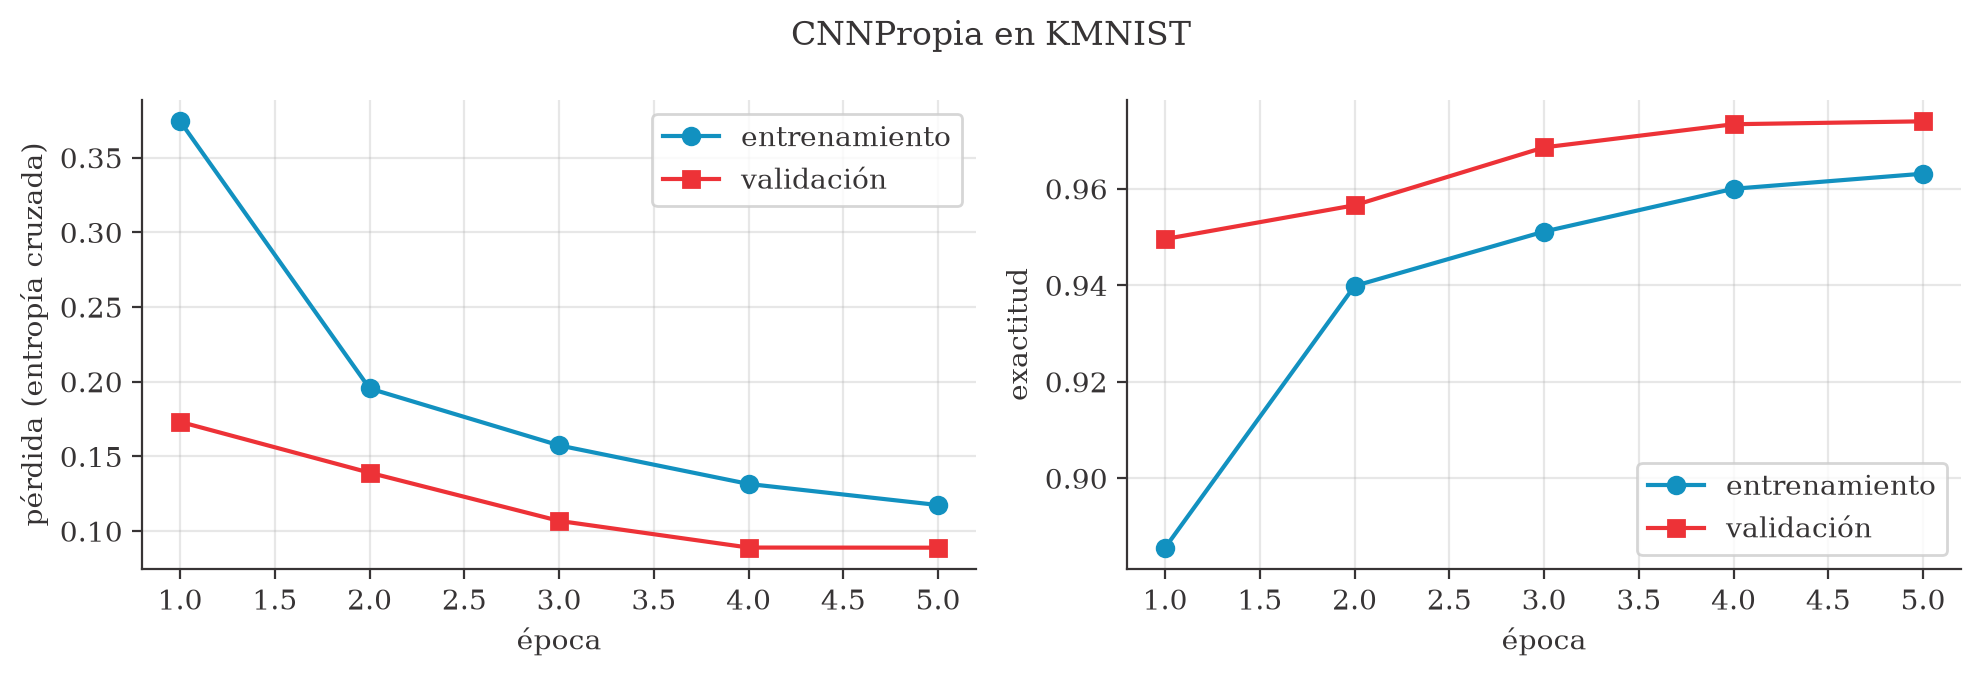
\includegraphics[width=\linewidth]{figuras/f03_curvas_cnnpropia.png}\par
      {\fontsize{7pt}{8.6pt}\selectfont Validación \cifraaccVal\,\%; la brecha entrenamiento--validación es de unos 0,9 pts: no hay sobreajuste aún.\par}
    \end{column}
  \end{columns}
\end{frame}

%% ------------------------------------------------------------------ 6
\begin{frame}{Resultado en prueba: \cifraaccTest\,\%}{\cifraerrTest{} errores de 10\,000; la validación daba \cifraaccVal\,\%}
  \begin{columns}[T,onlytextwidth]
    \begin{column}{0.40\textwidth}
      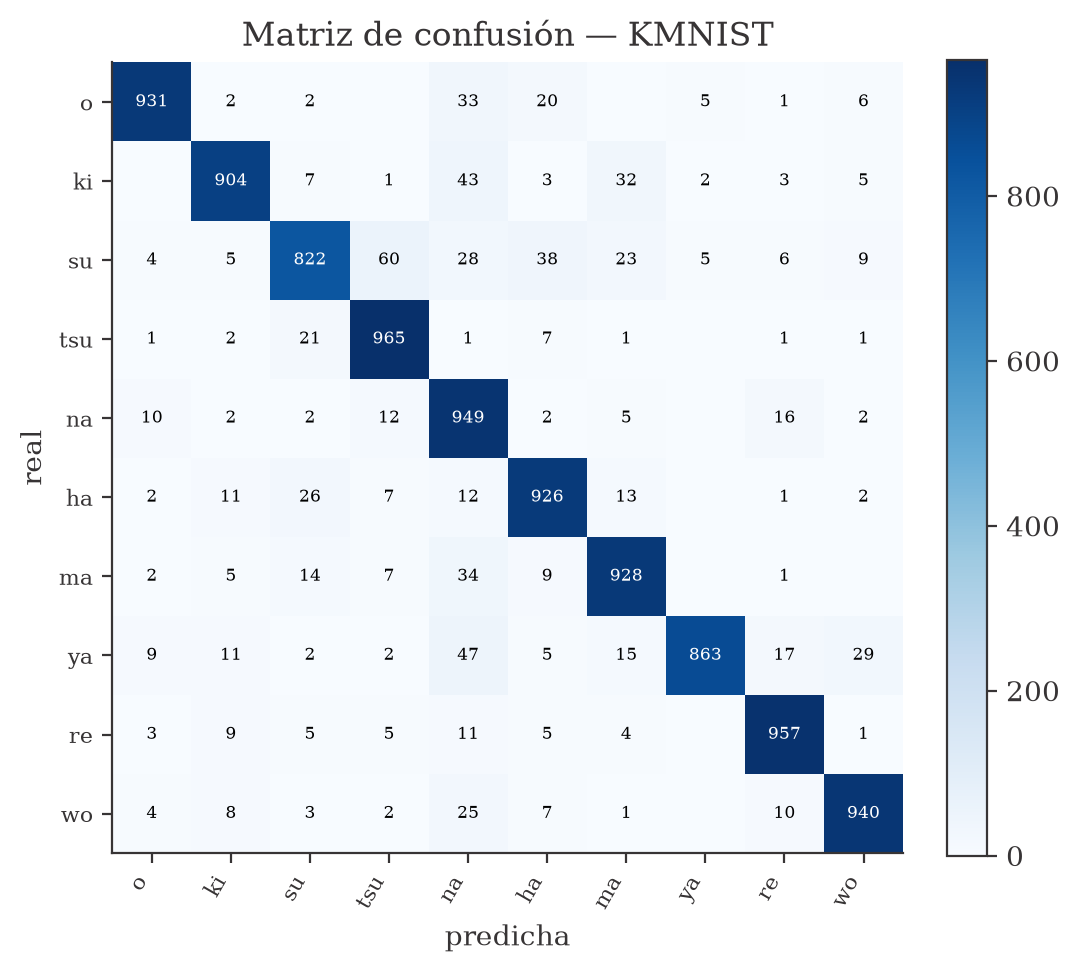
\includegraphics[width=\linewidth]{figuras/f04_matriz_confusion.png}
    \end{column}
    \begin{column}{0.58\textwidth}
      \cifraGrande{\cifraaccVal\,\%}{validación}{UDBlue}\hfill\cifraGrande{\cifraaccTest\,\%}{prueba}{UDRed}\hfill\cifraGrande{\cifrabrechaValTest\pts}{brecha}{UDGold}
      \vspace{0.18cm}
      \UDCard{white}{UDBorder}{\cardtitle{UDBlue}{La brecha no es un error}{\fontsize{7.2pt}{8.8pt}\selectfont
        Se repite con 5 semillas y \textbf{no} aparece en MNIST ni FashionMNIST. La validación sale del mismo reparto que el entrenamiento; la prueba oficial de KMNIST es más difícil (hipótesis: variantes de escritura solo en prueba). Para reportar rendimiento, \textbf{la prueba}.\par}}
    \end{column}
  \end{columns}
\end{frame}

%% ------------------------------------------------------------------ 7
\begin{frame}{Los errores: variantes de un mismo carácter}{Par más confundido: \textit{su} $\to$ \textit{tsu} (\cifraparN{} veces; al revés, \cifraparInv)}
  \begin{center}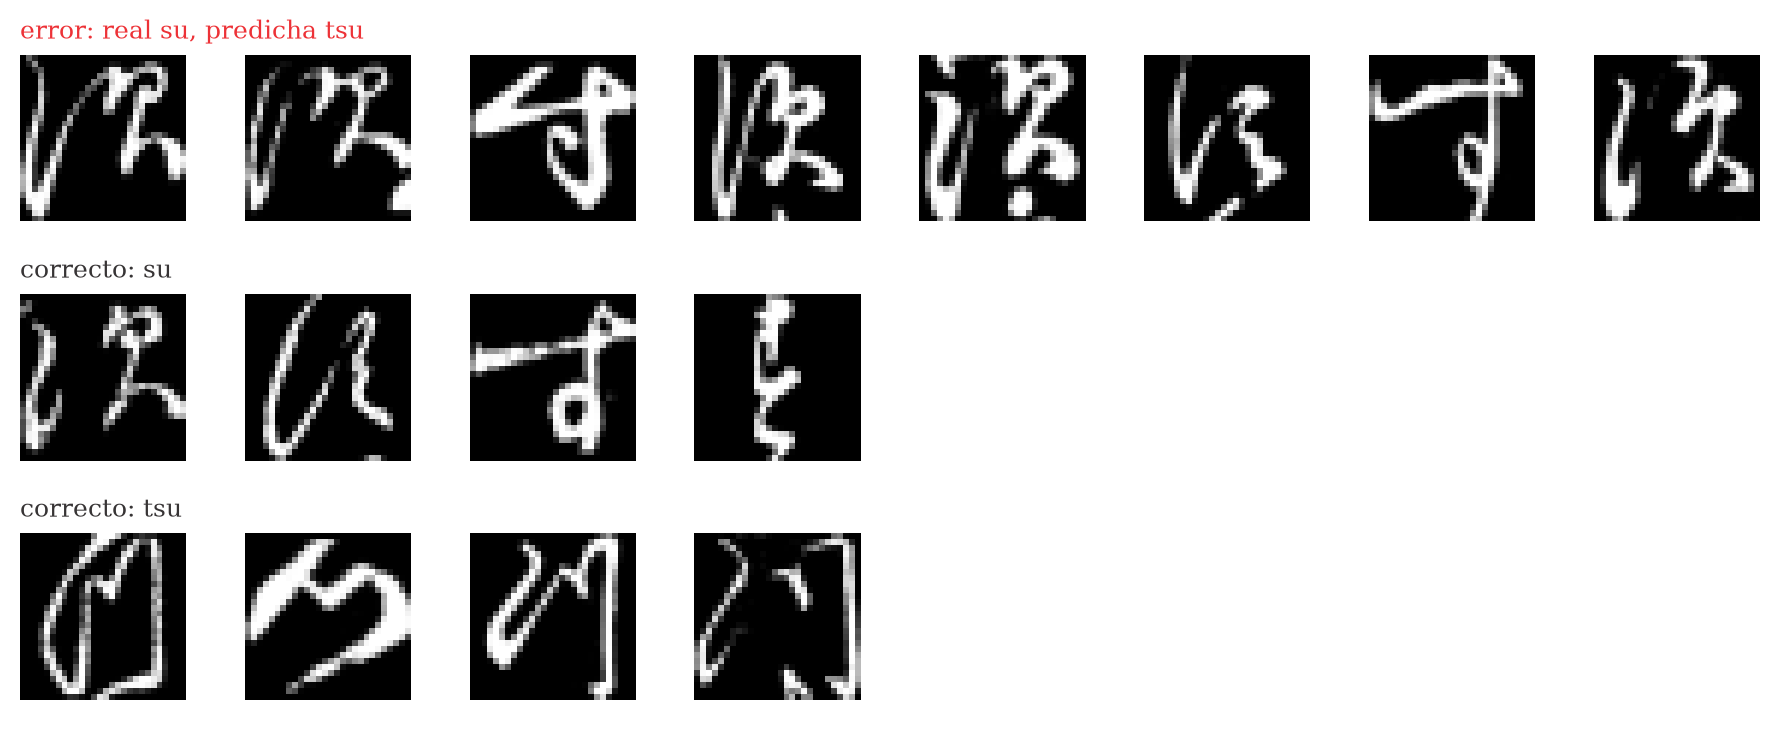
\includegraphics[width=0.86\linewidth]{figuras/f05_par_confundido.png}\end{center}
  \vspace{-0.1cm}
  {\fontsize{7.3pt}{9pt}\selectfont
  \textit{su} es la clase más difícil (\cifraclasePeorAcc\,\%). Los \textit{su} mal leídos son una \textbf{variante cursiva} distinta de la dominante y se parecen a grafías de \textit{tsu}: hay variación \textbf{dentro} de la clase, no desbalance. La confusión es asimétrica; \textit{na} actúa también como ``atractor'' (\textit{ya}, \textit{ki}, \textit{ma} $\to$ \textit{na}).\par}
\end{frame}

%% ------------------------------------------------------------------ 8
\begin{frame}{Aumento de datos: regulariza, pero no mejora}{Desplazamiento de $\pm2$ px, 5 semillas con el mismo orden de lotes}
  \begin{center}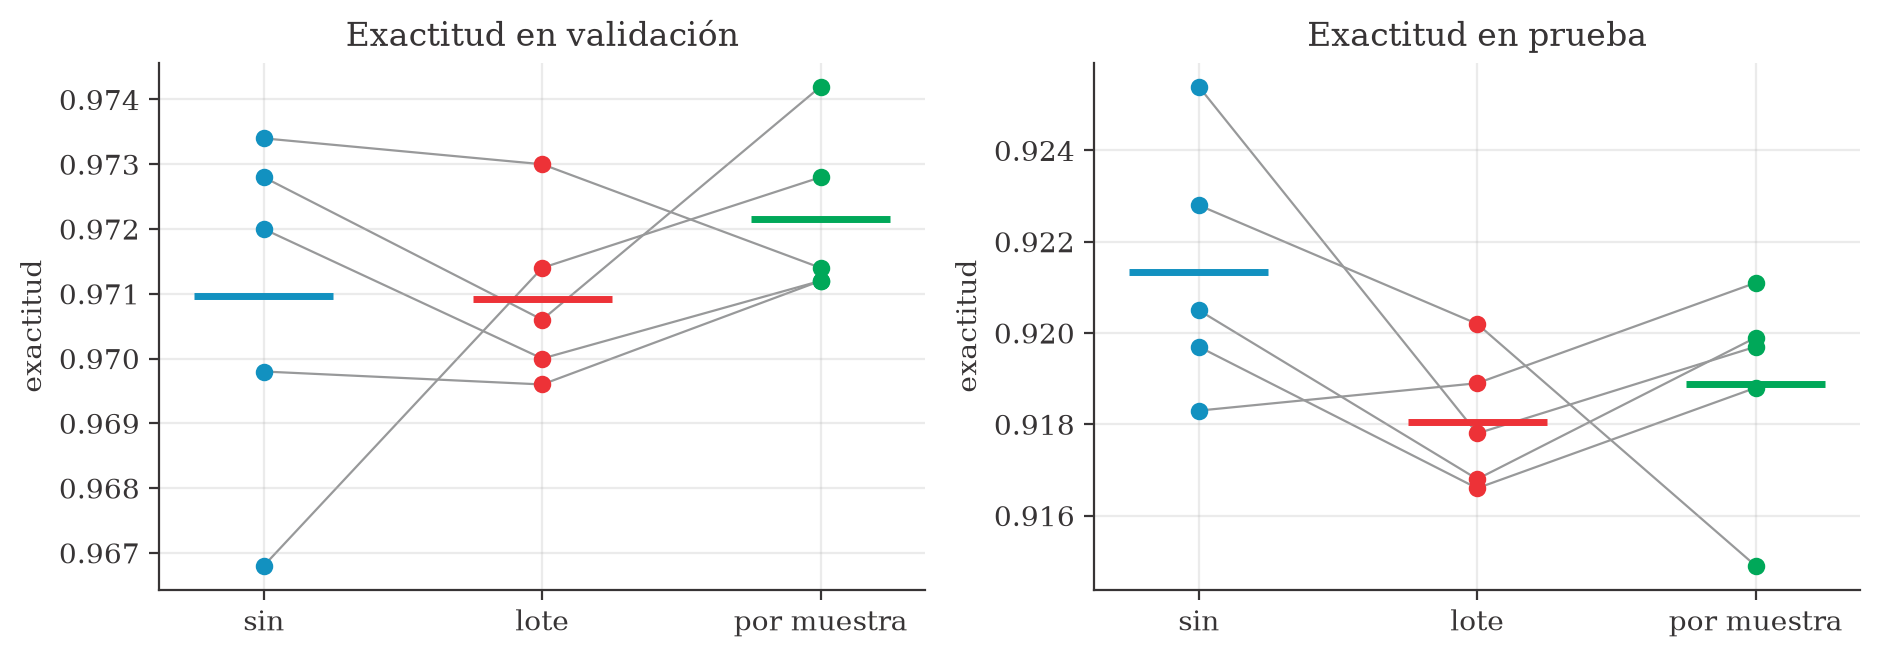
\includegraphics[width=0.93\linewidth]{figuras/f08_aumento_semillas.png}\end{center}
  \vspace{-0.15cm}
  \begin{columns}[T,onlytextwidth]
    \begin{column}{0.48\textwidth}
      {\fontsize{7.2pt}{8.8pt}\selectfont
      \textbf{Prueba} frente a ``sin aumento'': lote \cifraaugLoteTe\pts, por muestra \cifraaugMuestraTe\pts. \textbf{Validación}: \cifraaugLoteVal\pts{} y \cifraaugMuestraVal\pts. Dentro del ruido entre semillas.\par}
    \end{column}
    \begin{column}{0.48\textwidth}
      {\fontsize{7.2pt}{8.8pt}\selectfont
      La brecha entrenamiento--validación baja de 0,90 a $\approx$ 0,2 pts. Con 15 épocas: \cifralargoValDif\pts{} en validación y \cifralargoTeDif\pts{} en prueba. \textbf{Resultado negativo, reportado tal cual.}\par}
    \end{column}
  \end{columns}
\end{frame}

%% ------------------------------------------------------------------ 9
\begin{frame}{Extra: ablación y profundidad}{3 semillas pareadas; Dropout ayuda y la red base estaba subajustada}
  \begin{center}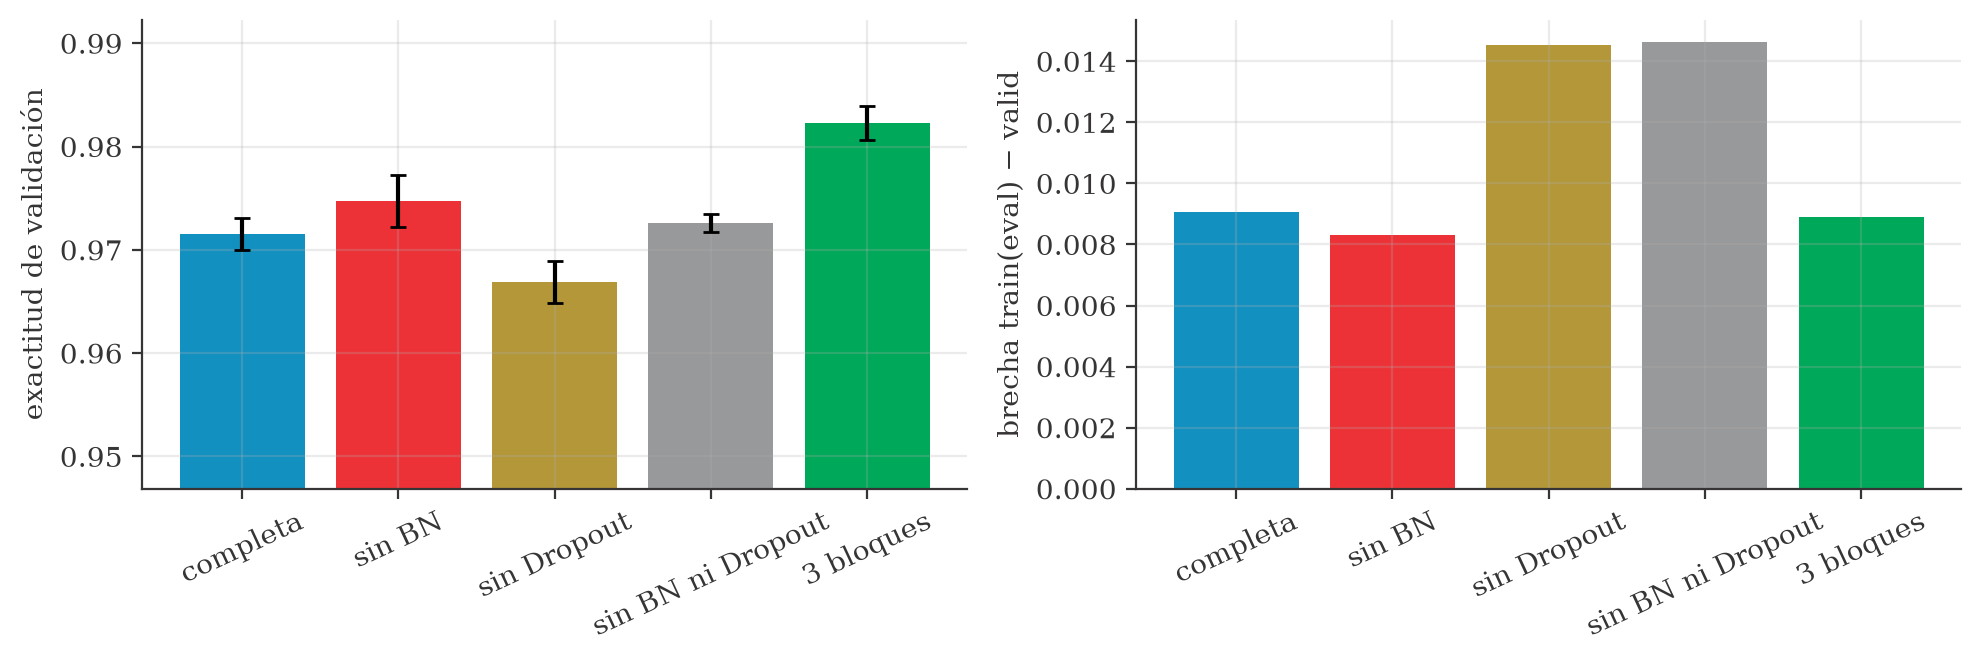
\includegraphics[width=0.96\linewidth]{figuras/f09_ablacion.png}\end{center}
  \vspace{-0.15cm}
  {\fontsize{7.2pt}{8.8pt}\selectfont
  Sin Dropout: validación \cifraablDropVal\pts, prueba \cifraablDropTe\pts, brecha \cifraablDropBrecha\pts. Sin BatchNorm: cambios de \cifraablBnVal{} y \cifraablBnTe\pts{} (ruido). \textbf{Tercer bloque: \cifraablTresVal{} en validación y \cifraablTresTe\pts{} en prueba} con 8\,704 parámetros más y sin crecer la brecha.\par}
\end{frame}

%% ------------------------------------------------------------------ 10
\begin{frame}{Extra: la convolución importa; KMNIST es particular}{Mismas condiciones, 3 semillas}
  \begin{columns}[T,onlytextwidth]
    \begin{column}{0.49\textwidth}
      \UDCard{white}{UDBorder}{\cardtitle{UDBlue}{Líneas base (prueba)}{\fontsize{7.2pt}{9pt}\selectfont
        MLP del docente (101\,770 par.): \textbf{\ciframlpTe\,\%}\par
        CNN del docente (12\,810 par.): \textbf{\cifracnnDocTe\,\%}\par
        CNNPropia (20\,586 par.): \textbf{\cifracnnPropTe\,\%}\par\vspace{0.05cm}
        La CNN pequeña supera al MLP con 8 veces menos parámetros, y el MLP memoriza (brecha 3,1 pts).\par}}
    \end{column}
    \begin{column}{0.49\textwidth}
      \UDCard{UDLightGray}{UDGold}{\cardtitle{UDGold}{La misma red en tres conjuntos}{\fontsize{7.2pt}{9pt}\selectfont
        \begin{tabular}{@{}lrrr@{}}
          & val. & prueba & brecha\\\midrule
          MNIST & \cifradsMNISTVal & \cifradsMNISTTe & \cifradsMNISTGap\\
          FashionMNIST & \cifradsFashionMNISTVal & \cifradsFashionMNISTTe & \cifradsFashionMNISTGap\\
          KMNIST & \cifradsKMNISTVal & \cifradsKMNISTTe & \textbf{\cifradsKMNISTGap}\\
        \end{tabular}\par\vspace{0.05cm}
        Solo KMNIST tiene una brecha validación--prueba apreciable.\par}}
    \end{column}
  \end{columns}
  \vspace{0.2cm}
  {\fontsize{7.2pt}{8.8pt}\selectfont\textbf{Tasa de aprendizaje} (2 épocas, 1 semilla): $10^{-1}$: \cifralrUno\,\%, $10^{-2}$: \cifralrDos\,\%, $10^{-3}$: \cifralrTres\,\%, $10^{-4}$: \cifralrCuatro\,\%, $10^{-5}$: \cifralrCinco\,\%. Control: con $\eta=10^{-1}$ la misma red da \cifralrUno\,\% con BatchNorm y \cifralrSinBnUno\,\% sin ella.\par}
\end{frame}

%% ------------------------------------------------------------------ 11
\begin{frame}{Conclusiones}{Lo que se aprendió, incluido lo que no funcionó}
  \begin{columns}[T,onlytextwidth]
    \begin{column}{0.48\textwidth}
      \UDCard{white}{UDBorder}{\cardtitle{UDBlue}{Lo que funcionó}{\fontsize{7.5pt}{9.2pt}\selectfont
        \begin{itemize}\setlength{\itemsep}{1pt}
          \item \cifraaccTest\,\% en prueba con 20\,586 parámetros.
          \item Dropout y un tercer bloque (+\cifraablTresTe\pts).
          \item CNN pequeña $\gg$ MLP con menos parámetros.
        \end{itemize}\par}}
    \end{column}
    \begin{column}{0.48\textwidth}
      \UDCard{UDLightGray}{UDRed!60}{\cardtitle{UDRed}{Lo que hay que saber}{\fontsize{7.5pt}{9.2pt}\selectfont
        \begin{itemize}\setlength{\itemsep}{1pt}
          \item Validación $\neq$ prueba en KMNIST (\cifrabrechaValTest\pts).
          \item El aumento no mejoró; solo regularizó.
          \item Errores = variantes cursivas, no desbalance.
        \end{itemize}\par}}
    \end{column}
  \end{columns}
  \vspace{0.2cm}
  {\fontsize{7.3pt}{9pt}\selectfont\textbf{Limitaciones.} 3 a 5 semillas, 5 épocas, una arquitectura base y una partición de validación fija: las diferencias de décimas de punto no son concluyentes. \textbf{Siguiente paso:} rotaciones o deformaciones elásticas y más épocas.\par}
\end{frame}

\UDcierre{Juan Felipe Rodríguez Galindo}
         {Maestría en Ciencias de la Información\\y las Comunicaciones}
         {Inteligencia Computacional Aplicada}

\end{document}
